\documentclass{article}

\usepackage[utf8]{inputenc}
\usepackage{enumitem}
\usepackage{graphicx}
\usepackage{tikz, amsmath, amssymb, gensymb}
\usepackage[english]{babel}
\usepackage{blindtext}
\usepackage[margin=1in]{geometry}
\usepackage[final]{pdfpages}
\setboolean{@twoside}{false}

\begin{document}

\begin{titlepage}
\newcommand{\HRule}{\rule{\linewidth}{0.5mm}}

\center

\textsc{\huge University of Waterloo}\\[3cm]
\textsc{\LARGE SE464}\\[1.5cm]
\textsc{\Large Section 001}\\[1.5cm]

\HRule \\[0.75cm]
{ \Huge \bfseries Deliverable 4: Project Architecture \& Design}\\[0.5cm]
\HRule \\[2cm]

\Large Group 25 \\  [8cm]

{\Large \today}\\

\vfill
\end{titlepage}

\section{Metadata}
\textbf{Project:} ShuttleQL (Shuttle Queueing Logistics) \\
\textbf{Team Name:} Baddie Boys \\
\textbf{Team Members:}
\begin{itemize}
  \item Cheng Dong (c9dong)
  \item Zhaotian Fang (z23fang)
  \item Clement Hoang (c8hoang)
  \item Di Sen Lu (dslu)
\end{itemize}

\section{Introduction}
Around the world, recreational badminton clubs host regular sessions at set locations for club members to drop in and play at. Traditionally, many of the tasks related to the operation of the club are done manually with the combined effort of the club's executive staff. Sometimes these tasks are repetitive and tedious and may require a execs full attention for a significant period of time. Examples of these tasks include:
\begin{itemize}
\item Registering new club members
\item Checking in and out members during a club session
\item Scheduling members into courts for each rotation
\end{itemize}
ShuttleQL is an all-in-one badminton club management platform that aims to automate many of the tasks above. The web-based platform consists of two main components:
\begin{enumerate}
\item Mobile web-based dashboard for the club members
\item Desktop web-based administration panel
\end{enumerate}
The online platform will act as a communication hub to increase transparency between the execs and members as well, notifying members of particular events in real time.

\newpage
\section{Architectural description}

\subsection{Overview}
At a high-level, the architectural components can be split into two groups: online and offline. The offline components consist of the matchmaker and pigeon, while online components make up the rest. The online components can be further divided into four different layers, as shown in the table below \\
\begin{tabular}{ | l | l | }
\hline
Layer & Component(s) \\
\hline
A & Player dashboard, Admin panel \\
B & API Gateway \\
C & User, Session, Announcement, Match service \\
D & User, Session, Announcement, Match database \\
\hline
\end{tabular} \\ \\
The online components make up a modified version of the three-tiered pattern. The front, middle, and back tiers are represented by layers A, C, and D respectively. Layer A contains the two web-applications that provide the user interfaces for the players and admins. Layer C contains the application functionality, separated based on the kind of data that is being operated on as described by the service name. Layer D contains the application data access and storage capabilities in the form of different databases where each database contains a specific category of data, which maps 1:1 with a service in layer C. In terms of communication, layer A communicates with C through HTTP and C with D through an FRM called Slick.

The responsibility of layer B will be explained later when the report focuses on the architecture of the API gateway.

The online components also make up a layered style. If we assume the layers A to D are stacked from top to bottom,
then a layer acts as a server to the layers above and acts as a client to the layers below. For example, layer B, the API gateway provides a client API for the web-applications (layer A) to use. In addition, layer B is a client to layer C, which exposes an internal API for the API gateway to use. The advantage to this pattern is reuse in the sense that a change to a particular layer means that you only have to modify at most two layers, the layer directly above and below.

A client-server style is exhibited between layers A and B. Layer B, the API gateway acts as a server that provides a set of user-facing client APIs. It doesn't know the number or identities of clients that will use its API. On the other hand, layer A, the web applications act as the client in the sense that it needs to know the explicit identity of the server in order to utilize the server's provided API.

\subsubsection{Player and Administrator Frontend}
The Player and Administrator Frontend (layer A) are the two interfaces where users can interact with the ShuttleQL. The Player frontend provides users with the ability to view current matches, whereas the Admin frontend provides club executives with the ability to manage club sessions, users, court usage. The main patterns used in these implementations are Flux architecture for data flow in the front-end. The Flux architecture consists of actions, views, reducers, and stores. It is a one-way data flow pattern where views dispatch actions, which are handled by the reducers in order to update the store, and the changes are propagated back to the views from top to bottom. In the views component, several modules are depended on for rendering. Material UI provides aesthetically pleasing components for the user interface, Router handles the rendering logic based on the URL supplied by the client, and React provides HTML rendering logic. In the Actions component, Axios is a module used to make HTTP requests, and Token Manager is an internal module used to authorize outgoing HTTP requests. Finally, there is a Socket.io client that listens to broadcasts from Pigeon.

\subsubsection{User, Session, Match, and Announcement Service}
The User, Session, Match and Announcement services are internal services. Each service is associated with a data type and has its own associated store. The exception to the rule is match service, whose purpose is to access the data stored in match maker. The services are self-contained in the sense that internal services should never need to interact with each other. If there needs to be coordination between services in response to a user event, the API gateway will handle that responsibility. This structure is common in a microservice architecture. The advantage to this pattern is that it maximizes cohesion in each service since all application functionality deals with the same type of data. It also minimizes coupling since the services don't need to interact with each other.

\subsubsection{API Gateway}
The API Gateway (layer B) serves as the interface for the frontend (layer A) to communicate with the internal services (layer C). The API Gateway follows the facade pattern in the sense that it abstracts out the complicated chaining of network calls to different internal services into one simple API. Therefore, it doesn't contain any business logic.
For example, when the frontend tries to get a list of checked-in players, the API Gateway first calls the Session service and gets a list of user ids'. Using those user ids', the API Gateway makes a call to User service to get the user info for each of the user ids'. Finally the list of user infos is returned to the frontend.

\subsubsection{Matchmaker}
The match maker is a background process that manages the members that are playing and waiting during a club session. Periodically, the match maker is in charge of rotating members on and off the court so everyone gets a chance to play. A key step in this process is the algorithm which groups players into different matches on each court. The goal of the algorithm is to turn a group of players into a group of matches. This data-flow operation follows the batch-sequential style. Between the start and end product, the data takes on various intermediate representations as its transformed by one component and passed to the next.

\subsubsection{Pigeon}
Pigeon is the component that notifies subscribers about events that happen in ShuttleQL. It follows the publish/subscribe style of implicit invocation. The announcers are the internal services that publish changes to data. The subscribers are the frontend clients. Pigeon is composed of two parts: the Amazon SNS portion, and the Pigeon server. Announcers send publish requests to Amazon SNS which delegates to the Pigeon server. Then the Pigeon Server forwards the message to subscribers. The advantage of this style is that it decouples the announcers from having to know who the subscribers are since these subscribers can change at any time.

\subsubsection{Gandalf}
Gandalf acts as the middleware security layer between layers B and C. It provides access control to the system's sensitive internal services. It has no significant architecture.

\subsection{Functional Properties}
From deliverable 1, 5 mandatory and 4 bonus functional properties were mentioned. The system satisfies all 5 mandatory functional properties and 1 of the 4 bonus functional properties.

\subsubsection{Mandatory}
Three out of the five mandatory functional properties describe admin-level actions such as registering new club members, checking in/out players, and overriding the matchmaking algorithm. They are all accomplished in a similar way by the system. The admin-panel component on the client-side provides a user interface for the admin to perform these actions. Each action is then proxied through the API gateway server. From that point, depending on the data that's being changed, the gateway will delegate to a specific internal service. For example, registering new club members means that the gateway will delegate to user service in order to persist a new user into the database.

Another functional property is that the system also allows the current matches to be displayed for the user to see. This information needs to be surfaced on both the admin panel and player dashboard. Therefore, it needs to be able to call an API to fetch the matches, which API gateway provides. Internally, API gateway delegates to game service to actually fetch the matches. Once the results are returned to the client, the data is rendered in a visually pleasing manner for the user to see.

Finally, the last mandatory functional property is that the system must have a match making algorithm that allocates players to open badminton courts. The matchmaking background process in the system architecture has exactly this responsibility. It will maintain a queue of players and periodically rotate current players off and allocate players that have been waiting onto the badminton courts. The current state of the queue and the mapping of players to courts is exposed to the internal game service only.

\subsubsection{Bonus}
One bonus functional property that was implemented was the ability for executives to broadcast announcements to users. The system accomplishes this by first providing the UI for the admin to construct an announcement and broadcast it. In addition, the system handles transferring the announcement data from the client through the API gateway and to the internal announcement service, where it'll be persisted. In addition, the system supports real-time message passing to the client through the component pigeon. Therefore, once the announcement is received by the internal service, it can leverage pigeon to send the announcement in real time to all connected players where it will be shown by the player dashboard UI.

A bonus functional property that wasn't implemented is the ability for admins to send notifications to users once they are able to play. This was never followed through since the system instead supports showing the user's status in the session that updates in real time. This feature accomplishes the problem that the original functional property was trying to solve and more.

The other bonus functional properties, the ability to show a match history and to track match-making-rating of club members were dropped since the level of effort needed to extend the system architecture to support these properties was not realistic given the time constraints of the group.

One functional property that was implemented which wasn't mentioned is the ability to keep the client user interfaces updated in real time. This is supported by the system through pigeon, which would notify connected clients that certain data is stale and must be updated through a fresh fetch from the server. The need to support this property is because data such as a user's status in a session, and the current set of games can all change without interaction from the user. Since there's never a need for the user to trigger a refresh, the system must do the job for the user instead.

\subsection{Non-functional Properties}
\subsubsection{Dependability}
The first of the two mandatory non-functional properties that have to be met is dependability, which describes the reliability of the system. This property is satisfied if the system can maintain an uptime of 95\% or better for every 24 hours. This is accomplished by deploying all backend services using Ngrok. This third-party service not only deploys any backend service but also provides a user interface as a terminal or web app that exposes crucial metrics related to the service such as uptime, server load, etc. Therefore, we're able to monitor the uptime of all deployed services to ensure that the property is met.

\subsubsection{Portability}
Portability is the second mandatory non-functional property, which describes the ability of a system to execute on multiple platforms while retaining its functional and non-functional properties. The concrete requirement is for the system to satisfy the following functional properties on both Chrome and Safari for mobile and desktop platforms: player registration, player checkin/checkout, matchmaking, and displaying the current matches. The frontend architecture for the admin panel and player dashboard supports the property through its lack of reliance on Javascript APIs with strict browser support. In addition, the architecture is careful to include only external dependencies that have good browser support across multiple platforms (i.e. material-ui).

\subsubsection{Efficiency}
Efficiency is the first of two bonus non-functional properties, which describes the system's performance. Since system performance is a very general requirement, it was narrowed down to the performance of the matchmaking algorithm. More specifically, the requirement is that the algorithm should run in less than 5 seconds given a pool of 100 badminton players. In order to maximize the efficiency of the algorithm, it is important to decouple the component away from any services so the component can be run in the background on a separate machine, where the hardware specs of the machine can be upgraded to meet the performance requirements of the algorithm. In addition, the algorithm is structured to fetch all needed data before the algorithm begins in order to prevent the need to make networks calls in the middle of the algorithm, which hinders its performance.

\subsubsection{Evolvability}
Evolvability is the last bonus non-functional property, which describes how well the system adapts to new requirements to the software. In order to make the requirement more relevant based on the context of the product, the requirement was narrowed down to if the system supports badminton clubs with different number of courts and different game types for each court. In order to fufill this requirement, the matchmaking algorithm is designed to be agnostic to the number of courts and their types. In addition, the information about the badminton club is stored in a configuration file, decoupled from the application code. This allows easy modification by people without needing to understand the system's components and code.

\newpage
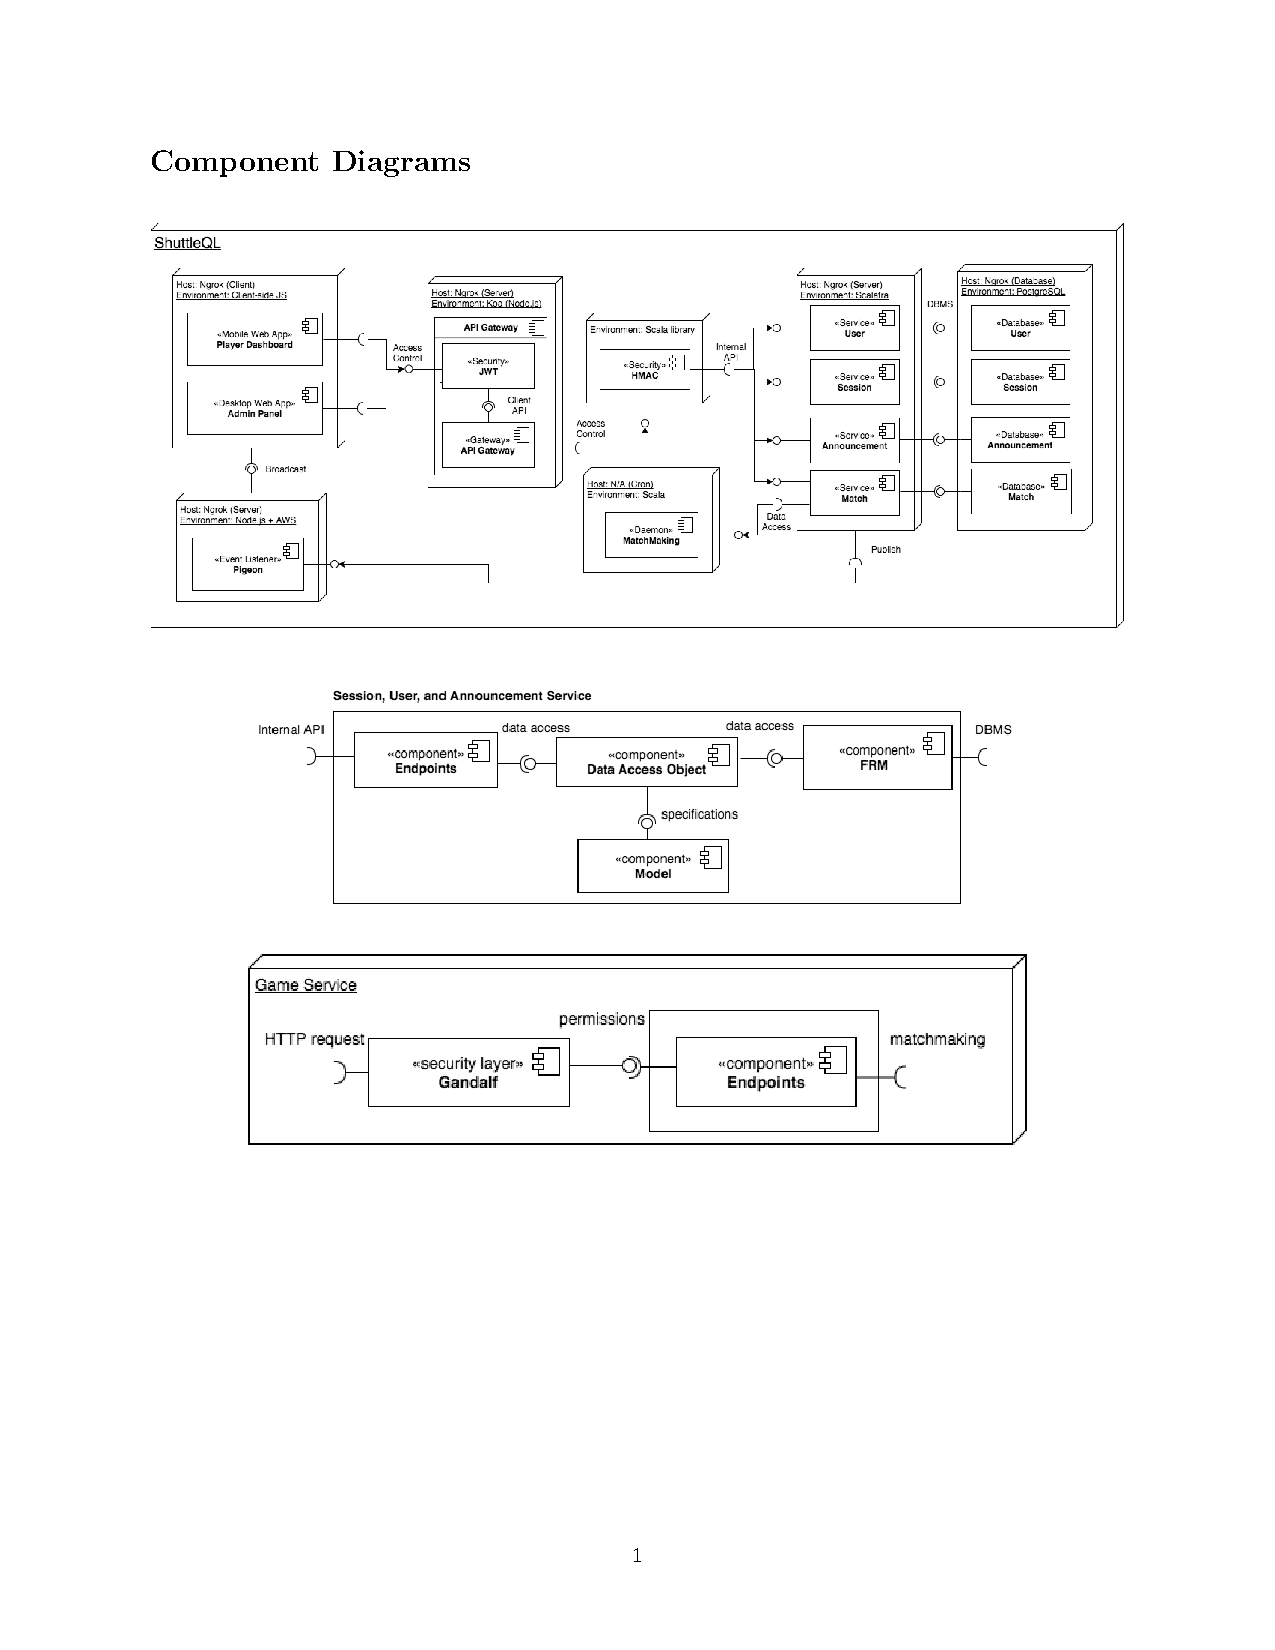
\includepdf[pages=-]{component_diagrams/d4_25_component_diagram.pdf}

\section{System design}

\subsection{Player and Administrator Frontend}
Player frontend is implemented using React, Redux, and Material UI. It's a single page application supported by React Router.

The Player frontend supports user sign in, as well as viewing announcements, matches, and profiles. In short, it's a readonly application, and has access to readonly APIs.

The Administrator frontend is built using the same tech stack as the Player frontend. However, it's has much more functionalities, including player registeration, session management, user management, and match override. It has access to all of the RESTful APIs.

React was chosen because of its ability to create reusable UI components, which makes web development faster, and more flexible. Redux provides a central storage for the state within the application, this makes components that share states to communicate in a much more efficient manner. Finally, Material UI was used to ensure a consistent look and feel within the application.

However, the disadvantage of using this setup is that it has a steep learning curve, as well as a long setup time. An alternative design would be to use a much more lighweight tool such as jQuery, and backbone. This lets the project to be setup much more quickly, but at the cost of maintenance and scalability once the codebase grows.

\subsection{API Gateway}
The API Gateway is written in Node.js using the Koa framework. The API gateway needs to perform complex chains of network calls to the internal services. The benefit of Koa is that performing asynchronous call chains is made relatively simple (for HTTP call aggregation). Also, since the heavy computations are done in the micro-services, then the lower performance of Node.js when compared to a compiled language is insignificant, and still suitable for the application.

One important aspect of the API Gateway is its security. The APIs needs to be able to verify that it is called by a valid client. To accomplish this, a Json Web Token (JWT) is used. Both the client and API Gateway maintains a common secret key. When the user logins in, the user id is encrypted using the secret key, and stored in local storage. During each API call, the encrypted id is appended to the header of the request, and the API Gateway decrypts id to verify that the client is valid.

This method not only provide authorization to the API Gateway, it also allows the client to keep a persistent session for the users.

The JWT protocol was chosen because it's simple, and quick to implement. It also provides sufficient security measure for the system. An alternative, and more complicated design would be to use a public key encryption such as RSA instead of a secret key encryption. A public key encryption protocal provide security to multiple clients, by providing each trusted client its own public key. This makes the system much more scalable in the future.

\subsection{Micro-services}
The announcement, user, match, and session services are all written in Scala using the Scalatra web framework. Looking into the codebase for the aforementioned services, there will be files with recurring patterns in their naming:

\begin{itemize}
  \item $x$Servlet.scala
  \item $x$DAO.scala
  \item $x$.scala
\end{itemize}

where $x$ approximately refers to the name of the service (i.e. User). This pattern is chosen due to the clear separation of concerns. $x$Servlet.scala contains the public API. $x$DAO.scala is data access object for $x$.scala, the model. Each microservice has its own related PostgreSQL database and it interfaces with the database through Slick, a FRM. This tech stack was chosen since they play well together.

\subsection{MatchMaker}
The match maker is a Scala component that resides in match service. Ideally, it should run as a background process (i.e. cron job), but for the sake of time, it was done this way instead. The responsibility of the match maker is to maintain state about each player in a session, whether they are playing on a specific court or whether they're waiting in queue. Periodically, it needs to rotate players on and off the court. During this process, it runs an algorithm to assign new players from the queue onto the courts. There are a variety of factors the algorithm considers, such as the length of time the player has been waiting, the player's skill level, and the player's court preference (singles or doubles). More generally, the algorithm transforms a list of players to a list of matches. Scala was the ideal language for this algorithm since it's functional and allows a series of data transformations to be written in a concise and readable manner.

\subsection{Gandalf}
Gandalf is the security layer within the microservices. Its purpose is to allow only trusted clients to use the API within the microservices. Gandalf was implemented as a scala package, and each mircoservice would import the package to use it. This minimizes code redundancy, since all the core logics are in a single package.

The trusted client (API Gateway), and each microservices all share a common secret key. Gandalf uses the HMAC protocal, where the client would select a random initialization vector (IV), and encrypts it, and sends both the encrypted and unenrypted version of the IV in each API request. Before the request reaches each microservice, Gandalf intercepts the request, and verifies that the IV is encrypted using the same secret key. This allows the microservices to verify that the request is coming from a trusted client.

An alternative design of Gandalf would be to use a public key encryption instead of a secret key encryption. As mentioned earlier in API Gateway, a public key encryption allows the system to be scaled to multiple clients, thus making the system more scalable. However, given the scope of the project, a secret key encryption provides sufficient security for the system, and is much easier to implement, therefore it was chosen over the public key encryption.

\subsection{Pigeon}
Pigeon Server is written in Node.js with Express and Socket.io. Socket.io is used to communicate between the server and subscribers, which are the front end clients. The choice in language and frameworks is because ShuttleQL required the ability to send real-time notifications to the front end clients. The only methods to achieve this are by long polling or websockets. The websocket approach was chosen as it has wide browser support, and prevents the need of constantly closing and re-opening connections. Consequently, Socket.io was chosen since it is one of the most supported libraries for websocket integration, and has good support for Node with Express. Pigeon Server is notified by Amazon SNS when actions occur in the micro-services. Amazon SNS was used because it provides an abstraction as well as a security layer for notifying Pigeon of events that happen. Without Amazon SNS, a custom security layer would have to be written for Pigeon.

\subsection{System Analysis}

\subsubsection{Coupling}
The system minimizes coupling through the micro-service architecture. Every backend service is a standalone application that is responsible for a specific set of actions. The backend services do not communicate with any other backend service and as a result, there are no dependencies between services. Each backend service is responsible for their own business logic and there is a clear separation of concern. In addition, the separation of the two frontend interfaces also decouples the business logic in the frontend. Rather than having a monolithic frontend application supporting both player and admin business logic, separating the two frontend interfaces better separates concerns and makes development easier.

\subsubsection{Adaptability to Future Requirements}
The two ways that the system could potentially change would be adding changes to the match making algorithm, changes to notifications and new functionalities pertaining to tournaments.

First, there will most likely be changes to the match making algorithm. ShuttleQL may be used by the UW badminton club and they will very likely have different requirements in the future to how matches are made. For instance, the number of courts can vary depending on the session and there may be special courts that only specific members can play on. Any varying business logic related to match-making can be altered in one method in the backend service, the match service. Thus, the system can easily adapt to changes in match-making, by adding the additional logic to one method and changing constants in a configuration file.

Second, the UW badminton club may want players to be notified via SMS messages when it is their turn to play rather than notifications within the application. This change can also be easily handled by the system. Right now in the match service, when a new set of matches are generated, a notification is sent to Pigeon to notify the players whether they are playing on a court. This can be replaced instead with a call to Twilio, a third-party SMS service that allows applications to send SMS messages via a phone number. Therefore, a change to SMS notifications can easily be handled by the system.

As of right now, the system only supports managing one badminton club. If a badminton club wants to use the system, they would have to own it (i.e. provide their own machines to host servers). This isn't ideal for the club since they have the responsibility to maintain the system even though they may not have technical staff. In the future, the system would have to be extended to support multiple badminton clubs so the badminton club doesn't have to own it. Instead, their only needs to ever be one copy of the system, which is managed by the development company (ShuttleQL).

\newpage
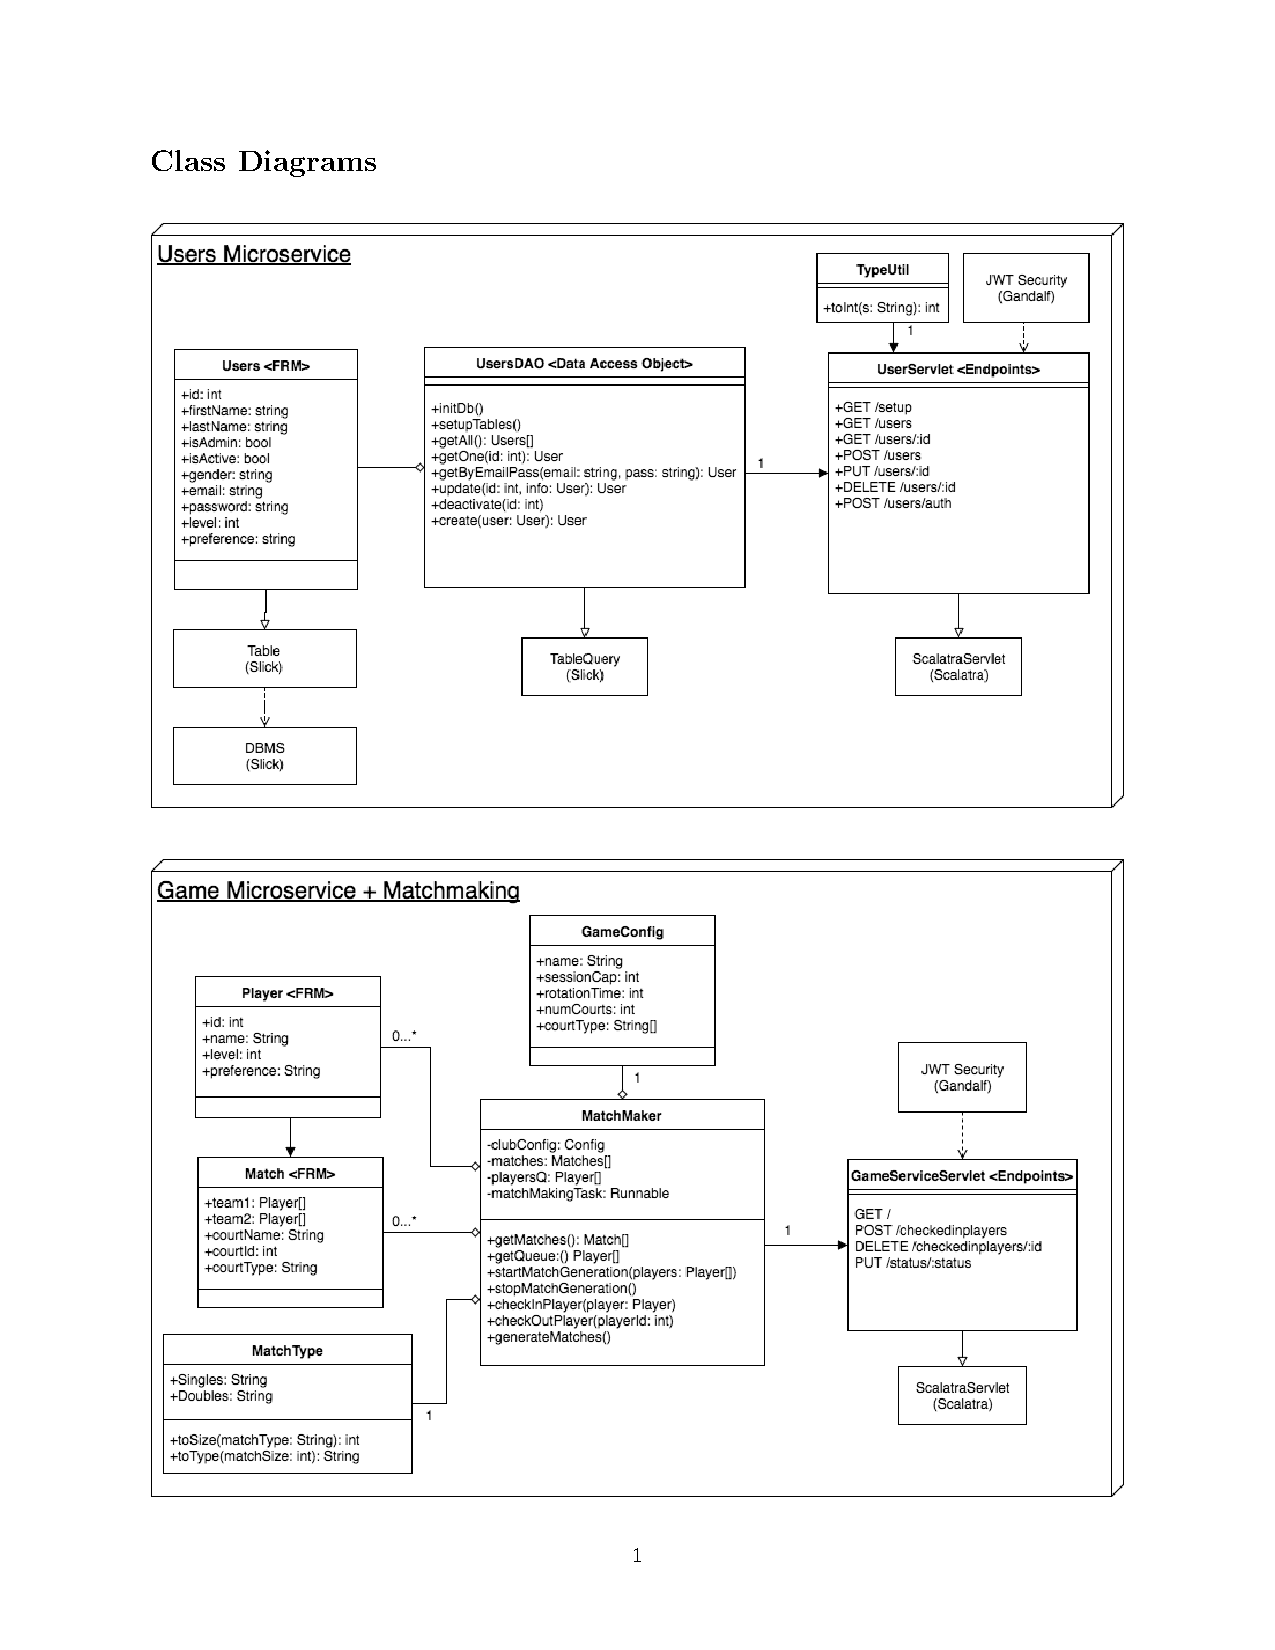
\includepdf[pages=-]{class_diagrams/d4_25_class_diagram.pdf}
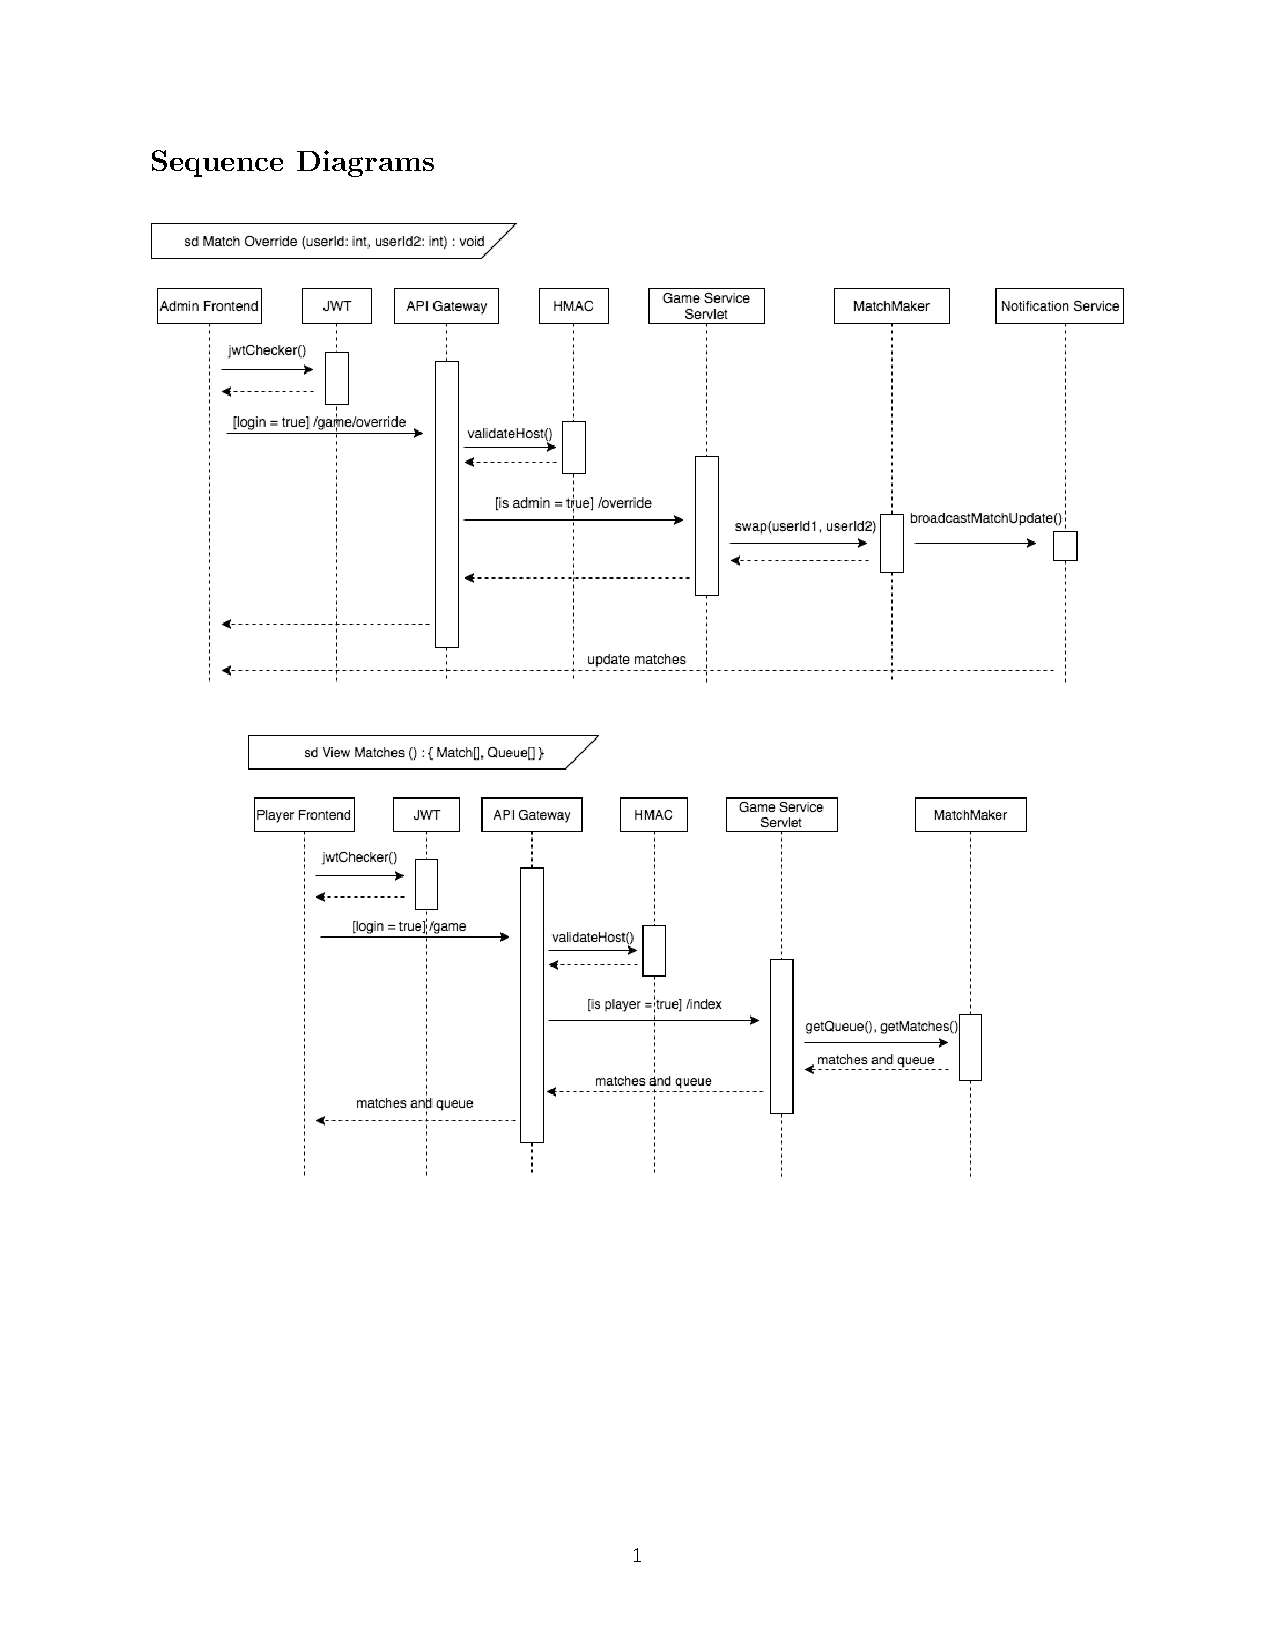
\includepdf[pages=-]{sequence_diagrams/d4_25_sequence_diagram.pdf}

\newpage
\section{Participation Journal}
Let $C,D,J,T$ represent that Clement Hoang, David (Cheng) Dong, Jason (Zhaotian) Fang, or Tony (Di Sen) Lu worked on a particular component/class.

Below is a table that maps each component/class to a list of 1 or more team members that worked on the component/class: \\
\begin{tabular}{ | l | c | c | l |  }
	\hline
    Component & Sub Component & Team Members & Total hours worked \\
    \hline
	Admin Panel & & C,J & 75 \\
	\hline
	Player Dashboard & & D,J & 50  \\
	\hline
	API Gateway & API & C,D,J,T & 10 \\
	& JWT & D & 15 \\
	\hline
	Gandalf & & D & 6  \\
	\hline
	User service & & C & 20 \\
	User database & & C & 4 \\
	\hline
	Session service & & T & 23 \\
	Session database & & T & 15 \\
	\hline
	Game service & & J,T & 7 \\
	Game database & & J & 3 \\
	\hline
	Announcement service & & J & 3 \\
	Announcement database & & J & 1 \\
	\hline
	Matchmaking & & C,J & 20 \\
	\hline
	Pigeon & & C & 12 \\
    \hline
\end{tabular} \\ \\

In the table below, the total number of hours worked per team member is shown across the entire system. \\
\begin{tabular}{ | l | l | }
	\hline
    Member & Total hours worked \\
    \hline
  	Clement Hoang & 86 \\
  	David (Cheng) Dong & 48.5 \\
	  Jason (Zhaotian) Fang & 89 \\
	  Tony (Di Sen) Lu & 40.5 \\
    \hline
\end{tabular}

\end{document}
